% Where Accuracy Is Lost: a stage-by-stage benchmark of TLE-based conjunction assessment
% IEEE conference format (IEEEtran). Compile: pdflatex main, bibtex main, pdflatex main x2 (or upload the folder to Overleaf).
% Every number traces to benchmarks/results/ in the ORCA repository; see MD/paper_draft.md for the long version.
\documentclass[conference]{IEEEtran}
\usepackage{iftex}
\ifXeTeX  % Tectonic / XeLaTeX: Times clone (IEEE body font)
  \usepackage{fontspec}
  \setmainfont{texgyretermes}[Extension=.otf, UprightFont=*-regular, BoldFont=*-bold,
    ItalicFont=*-italic, BoldItalicFont=*-bolditalic]
\else     % pdfLaTeX (e.g. Overleaf default): IEEEtran's own Times
  \usepackage[utf8]{inputenc}
\fi
\usepackage{cite}
\usepackage{amsmath}
\usepackage{graphicx}
\usepackage{booktabs}
\usepackage{url}

\begin{document}

\title{Where Accuracy Is Lost: A Stage-by-Stage Benchmark of TLE-Based Conjunction Assessment}

% TODO(authors): confirm order, add department, university and e-mail addresses.
\author{\IEEEauthorblockN{Surya Pratik, Abhinav Pentani, Shaik Saifuddin, Aditi Sharma}
\IEEEauthorblockA{\textit{Department (TODO), University (TODO)}\\
\textit{Supervised by Asish Kumar Dalai}\\
e-mail (TODO)}}

\maketitle

\begin{abstract}
Public two-line element sets (TLEs) are the only orbit data available for the whole catalogue, and open tools build conjunction-assessment pipelines on them, although NASA does not recommend TLE-based assessment for operations. We measure where such a pipeline loses accuracy. Each stage of an open pipeline, ORCA, is benchmarked on about 16,000 public TLEs against a dense reference built from the same data. Snapshot screening at 1\,h and 100\,km sees only 1.0--1.2\,\% of the encounters closer than 10\,km during their pass, as a simple sampling law predicts. ORCA's propagator drifts about 300\,km from SGP4 in a day. Its single-window refinement finds the closest approach for 5--6\,\% of flagged pairs. Its collision-probability formula is off by exactly $1/\alpha^2$, so every high-risk label it produces is an artefact. End to end, it reports about 0.1\,\% of the close approaches. A corrected pipeline recovers them at about nine times the cost. Finally, we measure TLE position error from successive TLEs. It is strongly anisotropic and about 15 times larger in-track for Starlink. With the measured covariance almost no encounter is high-risk, while plausible assumed covariances give anywhere from none to hundreds: in a TLE pipeline the covariance model, not the geometry, decides the risk tier.
\end{abstract}

\begin{IEEEkeywords}
space situational awareness, conjunction assessment, two-line elements, SGP4, screening, time of closest approach, collision probability, benchmarking
\end{IEEEkeywords}

% ---------------------------------------------------------------------------------------------------------------------
\section{Introduction}

\subsection{Background and Motivation}
Close approaches between catalogued objects in low Earth orbit (LEO) are routine. Operators act when the probability of collision $P_c$ exceeds a threshold, commonly $10^{-4}$~\cite{nasa_ca_handbook2020,merz2019}. The only orbit data freely available for the whole public catalogue are two-line element sets (TLEs), so public services and open tools build conjunction pipelines on them, from CelesTrak's SOCRATES~\cite{kelso2005socrates} to recent open-source screeners~\cite{sonawane2026}. NASA's handbook does not recommend TLE-based assessment for operations, ``because the TLE accuracy is not sufficient''~\cite{nasa_ca_handbook2020}. How much accuracy is lost, and at which stage of a pipeline, is rarely measured.

\subsection{Problem Statement}
A TLE pipeline has four stages: propagation, screening, refinement of the time of closest approach (TCA), and collision probability with a risk tier. Each stage rests on a choice the user does not see: the propagator, the screening step and radius, the refinement method, the $P_c$ formula, and the position covariance that TLEs do not carry. Errors compound. An encounter missed by screening never reaches the $P_c$ stage, and a $P_c$ computed with an unsupported covariance yields a confident tier without physical meaning.

\subsection{Research Gap}
Existing work compares screening tools on the public catalogue~\cite{georgeharvey2011}, defines screening accuracy requirements~\cite{auman2025}, counts conjunctions missed by orbit filters~\cite{woodburn2009}, compares $P_c$ formulas in isolation~\cite{alfano2007review,li2022review}, and shows that snapshot screening misses collisions in a synthetic debris setting~\cite{medhin2026}. Open TLE pipelines report speed but not accuracy~\cite{sonawane2026}. We found no measurement of (i) snapshot-screening recall on public TLEs as a function of step, radius and relative velocity, (ii) stage-by-stage accuracy loss in one working pipeline end to end, or (iii) the effect of measured versus assumed covariance on the tiers users see.

\subsection{Contributions}
\begin{enumerate}
\item A recall sweep of snapshot screening on public TLEs. A 1\,h / 100\,km screen sees 1.0--1.2\,\% of encounters closer than 10\,km, following the sampling law $2r/(v\Delta t)$.
\item A stage-by-stage audit of a working open pipeline, with a validated correction. The correction is now that pipeline's production engine.
\item A measured TLE covariance and its effect. On the same encounters, assumed covariances give 0 to $\sim$500 HIGH-tier events per 2,000 objects per day; the measured one gives 0--4.
\end{enumerate}

% ---------------------------------------------------------------------------------------------------------------------
\section{Preliminaries}

\subsection{TLE-Based Orbit Representation}
A TLE holds \emph{mean} elements fitted with the SGP4 theory. Using them with any other model degrades the prediction~\cite{hoots1980str3}, and SGP4 first converts the published Kozai mean motion to Brouwer's form~\cite{hoots1980str3,vallado2006revisiting}. Prediction accuracy is at the kilometre level~\cite{vallado2006revisiting}: the error is dominated by the along-track component~\cite{flohrer2009improving} and grows by about 1.5\,km per day against precise orbits~\cite{levit2011improved}. TLEs carry no covariance~\cite{flohrer2009improving,nasa_ca_handbook2020}.

\subsection{Conjunction Screening}
All-versus-all screening of $N$ objects involves $N(N-1)/2$ pairs, about $1.3\times10^8$ for $N=16{,}000$. Filters discard pairs that cannot meet~\cite{hoots1984,woodburn2009}. Snapshot screening instead propagates all objects on a grid $t_k=k\Delta t$ and, at each step, uses a k-d tree~\cite{bentley1975} to find pairs closer than a radius $r$. An encounter with miss distance $d$ and relative speed $v$ is guaranteed to be sampled only if
\begin{equation}
r \ge d + v\,\Delta t/2 .
\label{eq:capture}
\end{equation}
Otherwise it is caught with probability of about $2\sqrt{r^2-d^2}/(v\Delta t)$.

\subsection{Time of Closest Approach}
The TCA is a root of the range rate, $\Delta\mathbf r\cdot\Delta\mathbf v=0$, crossing from negative to positive. It can be found robustly by bracketing on a grid and refining with Brent's method~\cite{brent1973}. For straight-line relative motion $d^2(t)$ is exactly quadratic, so a parabola through three samples locates the TCA. A LEO pair has several approach minima per orbit, so a single minimisation over a long window can stop at any of them.

\subsection{Collision Probability and Risk Tiers}
In the short-term encounter model~\cite{akella2000,chan2008}, the miss vector $\mathbf m$ and the combined covariance $C$ are projected onto the plane normal to the relative velocity. $P_c$ is then the Gaussian mass inside the combined hard-body radius $R$:
\begin{equation}
P_c=\iint_{|\mathbf x|\le R}\frac{1}{2\pi\sqrt{|C|}}\,e^{-\frac12(\mathbf x-\mathbf m)^{\!\top}C^{-1}(\mathbf x-\mathbf m)}\,d\mathbf x .
\label{eq:pc}
\end{equation}
Foster's method integrates (\ref{eq:pc}) numerically~\cite{foster1992}. A Monte Carlo estimate needs about $(1-P_c)/(P_c\varepsilon^2)$ samples for relative error $\varepsilon$. Slow encounters break the model's assumptions~\cite{coppola2012,alfano2009mc}. Tiers use $P_c$ thresholds of $10^{-4}$, $10^{-5}$, $10^{-6}$ and $10^{-7}$.

% ---------------------------------------------------------------------------------------------------------------------
\section{Literature Review}

\subsection{TLE Accuracy}
SGP4 was published in Spacetrack Report~\#3~\cite{hoots1980str3} and its reference code revisited by Vallado et al.~\cite{vallado2006revisiting}. Flohrer et al. derived TLE uncertainties by orbit class: LEO averages at epoch are 0.10, 0.47 and 0.13\,km radial, along-track and cross-track~\cite{flohrer2009improving}. Kelso showed that TLE-to-TLE consistency approximates the true error but underestimates it near epoch~\cite{kelso2007validation}. Levit and Marshall reduced error growth by fitting TLE histories~\cite{levit2011improved}. Starlink satellites manoeuvre every one to two days in their operational shells~\cite{liu2024maneuver}, and continuous low-thrust propulsion makes them hard to predict~\cite{lang2025starlink}; operator ephemerides are public~\cite{ou2025starlink}, and CelesTrak publishes elements derived from them~\cite{celestrak_supgp}.

\subsection{Conjunction Screening}
Hoots et al. introduced the apogee--perigee, orbit-path and time filters~\cite{hoots1984}. Woodburn et al. showed these need pads, losing 4 of 5,338 conjunctions without them~\cite{woodburn2009}. Parallel and sieve methods followed~\cite{healy1995,alarcon2002}. Sort-and-sweep~\cite{george2011} and k-d tree or spatial-hash screeners~\cite{budianto2014} avoid sampling misses by screening swept volumes. George and Harvey compared six tools on public TLEs; tools missed 33 to 326 conjunctions because of filter pads~\cite{georgeharvey2011}. Stevenson et al. benchmarked learned screening on simulated data~\cite{stevenson2023}, and Medhin and Servadio measured the blindness of snapshot grids in a synthetic setting~\cite{medhin2026}. Sonawane screened the CelesTrak catalogue with a grid and a k-d tree and reported speed-ups but not recall~\cite{sonawane2026}.

\subsection{TCA and Collision Probability}
Alfano and Negron fitted cubic polynomials to separation histories~\cite{alfano1993}. Short-term $P_c$ methods~\cite{foster1992,akella2000,patera2001,alfano2005numerical,chan2008} are reviewed in~\cite{li2022review}. Alfano compared Foster, Chan, Patera and Alfano on about 60,000 cases and found all of them accurate to at least two significant figures~\cite{alfano2007review}. Monte Carlo test cases~\cite{alfano2009mc}, NASA's CARA tools~\cite{cara_tools} and Orekit~\cite{orekit12} support validation. Covariance for TLEs comes from look-up tables~\cite{flohrer2009improving} or from TLE histories, as in COVGEN~\cite{peterson2001covgen}.

\subsection{Gap}
Screening speed, filter design, tool agreement and $P_c$ formulas in isolation are well covered. Recall against sampling on public TLEs, stage-wise accuracy inside a working pipeline, and the effect of measured covariance on tiers are not.

% ---------------------------------------------------------------------------------------------------------------------
\section{Methodology}

\begin{figure*}[t]
\centering
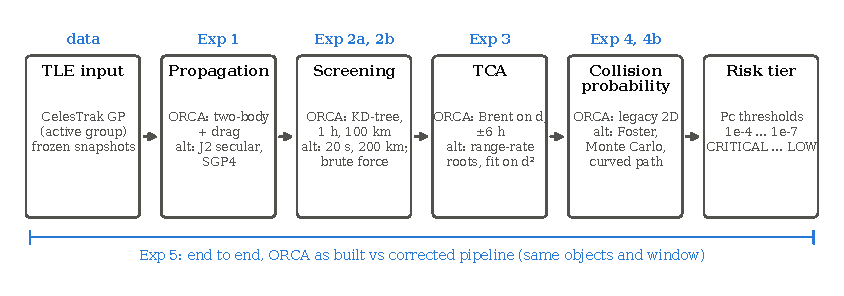
\includegraphics[width=\textwidth]{figures/fig_pipeline.pdf}
\caption{The pipeline and where each experiment intervenes. Each box gives ORCA's original method and the alternatives compared. Exp.~5 runs both complete pipelines on the same objects and window.}
\label{fig:pipeline}
\end{figure*}

\subsection{ORCA and the Benchmark Harness}
ORCA is an open conjunction-assessment application (FastAPI back end, React front end) that works only from public TLEs. As built, it propagated with a two-body model plus exponential drag. It screened every 1\,h with a k-d tree at 100\,km and refined each flagged pair with one bounded Brent minimisation over $\pm6$\,h. It then computed a 2D $P_c$ under an isotropic covariance $\sigma=0.5\,\mathrm{km}+2\,\mathrm{km/day}\times$ TLE age and assigned tiers (Fig.~\ref{fig:pipeline}). The harness swaps one stage at a time and calls ORCA's own functions wherever ORCA itself is measured. A frozen copy of the original code keeps that baseline reproducible.

\subsection{Data and Environment}
Table~\ref{tab:data} lists the data and environment. Conjunction experiments use three random subsets of 2,000 LEO objects (apogee $\le2000$\,km, TLE at most 7 days old), all over the same 24\,h window.

\begin{table}[t]
\caption{Data and environment}
\label{tab:data}
\centering
\begin{tabular}{@{}ll@{}}
\toprule
Source & CelesTrak GP, group \texttt{active} (payloads)\\
Snapshots & 15,970 / 15,932 / 15,932 TLEs, 2026-10-14\\
Window & 24\,h from 2026-10-10 02:10 UTC\\
Populations & $3\times2{,}000$ LEO objects (seeds 1--3)\\
Software & Python 3.12, SciPy 1.18, sgp4 2.27\\
Hardware & Ryzen 9 5900HS, 15.4\,GB, single process\\
\bottomrule
\end{tabular}
\end{table}

\subsection{Experiments}
Table~\ref{tab:exp} summarises the five experiments.

\textbf{Exp.~1, propagation.} Three propagators are compared: ORCA's model, two-body with first-order $J_2$ secular rates on Brouwer elements (rates checked against SGP4's own to $10^{-5}$), and SGP4~\cite{rhodes_sgp4}. They are scored against two references: SGP4 of the same TLE (model consistency) and the object's next TLE (TLE-to-TLE). Errors are split into radial, in-track and cross-track (RIC) components, with robust spreads.

\textbf{Exp.~2, screening.} The reference propagates every object with SGP4 every 10\,s and collects all pairs within 200\,km. Each grid minimum is refined; by (\ref{eq:capture}) with $v\le16$\,km/s, every encounter below 10\,km is captured. A snapshot screen with step $\Delta s$ and radius $r$ \emph{detects} an encounter if it flags a sample during that encounter's own pass. Runtime of brute force and the k-d tree is compared on identical snapshots.

\textbf{Exp.~3, TCA.} Grid search, a parabola on $d^2$, bounded Brent, and Brent on the range rate are compared within $\pm60$\,s of each encounter. ORCA's $\pm6$\,h refinement is compared with root-finding of every minimum.

\textbf{Exp.~4, $P_c$.} ORCA's formula, Foster~\cite{foster1992}, the isotropic closed form and Monte Carlo (Clopper--Pearson intervals~\cite{clopper1934}) are compared under four covariances: ORCA's isotropic $\sigma$; an assumed in-track-dominant shape; the covariance measured in Exp.~1; and that covariance floored at ESA's at-epoch values~\cite{flohrer2009improving}.

\textbf{Exp.~5, end to end.} ORCA as built (A) is run alongside a corrected pipeline (B): SGP4, a 20\,s / 200\,km screen, range-rate root-finding and Foster.

\begin{table}[t]
\caption{Experiment design}
\label{tab:exp}
\centering
\begin{tabular}{@{}lll@{}}
\toprule
Exp. & Compared & Reference\\
\midrule
1 & 2-body+drag, 2-body+$J_2$, SGP4 & SGP4; next TLE\\
2 & steps 20\,s--1\,h, radii 10--200\,km & 10\,s SGP4 grid\\
3 & grid, $d^2$ fit, Brent, range-rate roots & root to $10^{-6}$\,s\\
4 & ORCA formula, Foster, MC & closed form; MC\\
5 & ORCA as built vs corrected & SGP4 near TCA\\
\bottomrule
\end{tabular}
\end{table}

% ---------------------------------------------------------------------------------------------------------------------
\section{Results and Discussion}

\subsection{Propagation}
Against SGP4 of the same TLE (Fig.~\ref{fig:prop}), ORCA's model drifts 83\,km at 6\,h, 303\,km at 24\,h and 2,920\,km at 7 days (medians over $\sim$15,160 LEO objects). Adding $J_2$ secular rates keeps the difference near 11\,km through 24\,h. Against the next TLE, SGP4's error at 5--7 days for non-Starlink objects has robust RIC spreads of 0.13, 14.6 and 0.21\,km. Along-track is thus about 100 times radial, and ORCA's isotropic 12.5\,km overstates the radial error about 90-fold. With three snapshots, the in-track spread grows from 0.16\,km at 0.3\,days to 14.6\,km at 6.3\,days. Starlink TLEs are about 15 times worse in-track, and SGP4's error for them grows with the fitted drag term B$^*$, consistent with thrust absorbed into the elements~\cite{lang2025starlink}.

\begin{figure}[t]
\centering
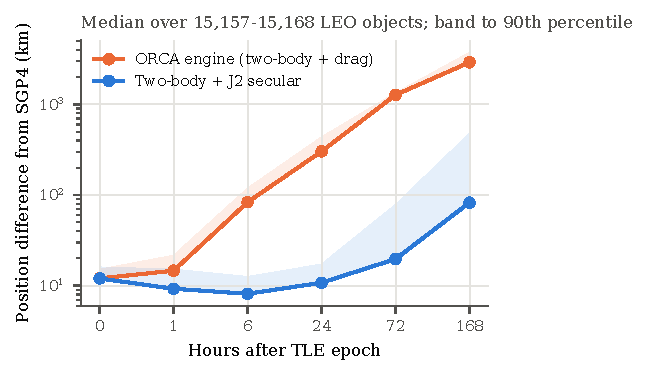
\includegraphics[width=\columnwidth]{figures/fig_propagation_r1.pdf}
\caption{Position difference from SGP4 of the same TLE (median; band to 90th percentile).}
\label{fig:prop}
\end{figure}

\subsection{Screening}
Brute force and the k-d tree return identical pair sets at every size. The k-d tree is 36 times faster at 1,000 objects and 173 times faster at 15,913, where it takes 8.5\,ms per step (Fig.~\ref{fig:runtime}). The spatial search is therefore cheap; recall is the problem (Fig.~\ref{fig:recall}).

\begin{figure}[t]
\centering
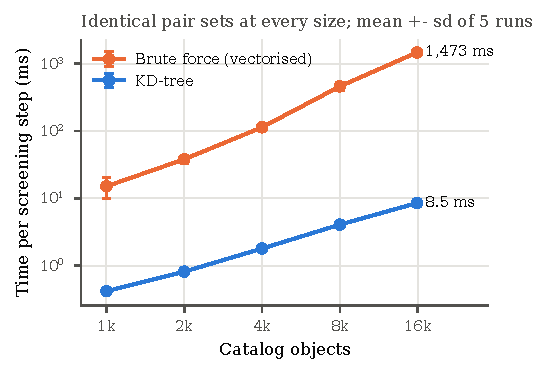
\includegraphics[width=\columnwidth]{figures/fig_screening_runtime.pdf}
\caption{Time per screening step, brute force against k-d tree, on identical SGP4 snapshots (mean $\pm$ s.d. of 5 runs).}
\label{fig:runtime}
\end{figure} Across 6,214--6,803 reference encounters per seed:
\begin{itemize}
\item a 1\,h / 100\,km screen detects 1.0--1.2\,\% of them during their pass;
\item a 1\,min / 100\,km screen detects about 41\,\%;
\item a 20\,s / 200\,km screen detects all of them, as (\ref{eq:capture}) guarantees.
\end{itemize}
Recall falls with relative speed: it is 100\,\% below 0.1\,km/s but under 1\,\% above 5\,km/s at ORCA's setting, matching $2r/(v\Delta t)$. As a result, ORCA's output was dominated by slow, co-orbital pairs.

\begin{figure}[t]
\centering
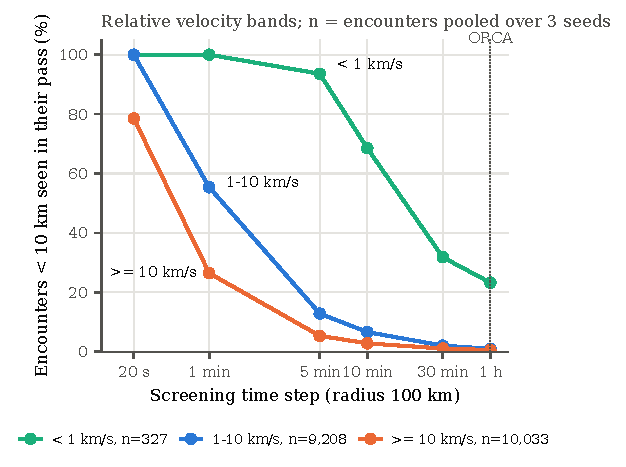
\includegraphics[width=\columnwidth]{figures/fig_screening_recall.pdf}
\caption{Share of encounters closer than 10\,km whose pass is sampled by a 100\,km screen, by relative velocity (three seeds pooled).}
\label{fig:recall}
\end{figure}

\subsection{Time of Closest Approach}
Grid search alone is a poor miss-distance estimator (Fig.~\ref{fig:tca}). Even a 1\,s grid errs by a median of 353\,m, because at 10\,km/s half a second is 5\,km. A parabola on $d^2$ from a 60\,s grid gives 0.84\,m with four evaluations. Brent on the range rate is exact to below a microsecond with nine. ORCA's single $\pm6$\,h minimisation finds the closest approach for only 5.4--6.1\,\% of the pairs it flags, because such a window contains about 15 approach minima. Root-finding every minimum finds all of them.

\begin{figure}[t]
\centering
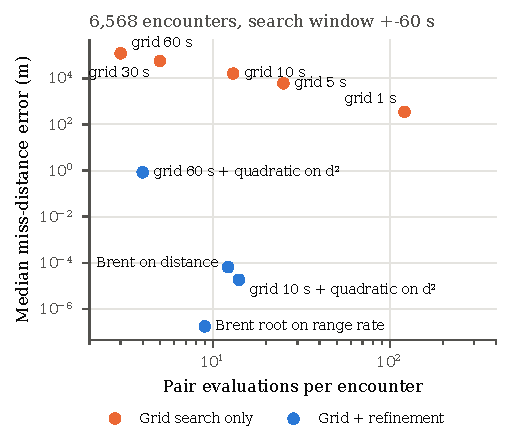
\includegraphics[width=\columnwidth]{figures/fig_tca_tradeoff.pdf}
\caption{Median miss-distance error against cost for TCA methods (6,568 encounters, window $\pm60$\,s).}
\label{fig:tca}
\end{figure}

\begin{figure}[t]
\centering
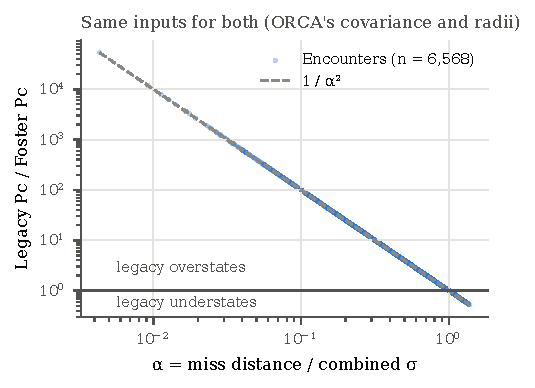
\includegraphics[width=\columnwidth]{figures/fig_pc_ratio.pdf}
\caption{ORCA's $P_c$ divided by Foster's, against $\alpha$ (same covariance and radii); the dashed line is $1/\alpha^2$.}
\label{fig:pcratio}
\end{figure}

\subsection{Collision Probability}
On identical inputs, ORCA's $P_c$ equals Foster's divided by $\alpha^2$ ($\alpha$ = miss/$\sigma$; Fig.~\ref{fig:pcratio}). Foster matches the closed form to $10^{-12}$ and Monte Carlo in 50 of 50 cases per seed. The consequences:
\begin{itemize}
\item every one of ORCA's 455--550 CRITICAL and HIGH events per seed is MEDIUM or LOW under Foster;
\item ORCA's ranking was effectively a miss-distance ranking (Kendall $\tau=0.87$), whereas Foster's is not ($\tau=0.41$--$0.43$);
\item at $P_c\approx10^{-6}$, Monte Carlo returned no hits up to $10^5$ samples and came within 15\,\% only at $10^8$ (Fig.~\ref{fig:mc}). The original plan of $10^3$--$10^5$ samples would have returned zero.

\begin{figure*}[t]
\centering
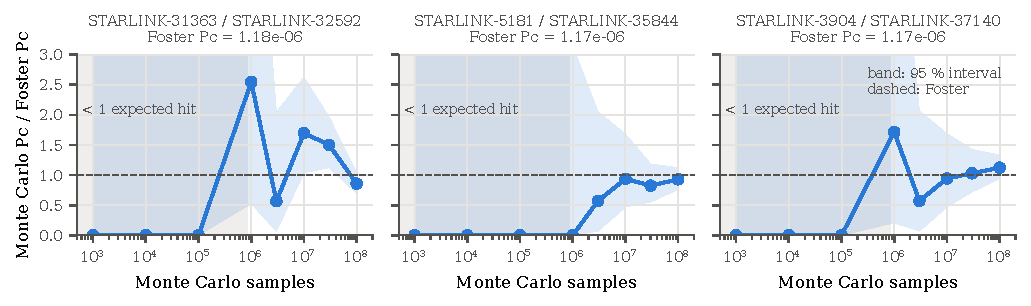
\includegraphics[width=\textwidth]{figures/fig_mc_convergence.pdf}
\caption{Monte Carlo $P_c$ divided by Foster's for the three highest-$P_c$ encounters ($P_c\approx1.2\times10^{-6}$), with 95\,\% Clopper--Pearson intervals. The grey region marks fewer than one expected hit.}
\label{fig:mc}
\end{figure*}
\end{itemize}
Within a single pass the straight-line model holds from 0.1\,km/s up; below that, with elongated covariance, it underestimates by about $6\times$.


\subsection{End to End, and the Covariance}
Table~\ref{tab:e2e} compares the two pipelines. ORCA as built finds 6--8 of about 6,500 encounters per seed and misreports miss distances by a median of about 90\,km. The corrected pipeline reproduces the reference to within one event per seed at nine times the runtime. Table~\ref{tab:tiers} shows that for these \emph{same} encounters the tiers depend on the covariance far more than on the method. It is now ORCA's production engine: on the full catalogue it finds about 426,000 approaches closer than 10\,km in a day, in 1.5--2 minutes.

\begin{table}[t]
\caption{End to end, seeds 1/2/3}
\label{tab:e2e}
\centering
\begin{tabular}{@{}lcc@{}}
\toprule
& A: as built & B: corrected\\
\midrule
Encounters $<$10\,km found & 8 / 6 / 7 & all\\
Median miss error & 90 / 98 / 85\,km & $<$1\,mm\\
Runtime (2,000 obj., 24\,h) & 2.6\,s & 24--25\,s\\
\bottomrule
\end{tabular}
\end{table}

\begin{table}[t]
\caption{HIGH-tier events per seed under each $P_c$ setting (same encounters)}
\label{tab:tiers}
\centering
\begin{tabular}{@{}lc@{}}
\toprule
$P_c$ formula and covariance & HIGH (and CRITICAL)\\
\midrule
ORCA formula, ORCA isotropic $\sigma$ & 455--550\\
Foster, ORCA isotropic $\sigma$ & 0\\
Foster, assumed in-track-dominant shape & 471--576\\
Foster, measured covariance & 0--3\\
Foster, measured, ESA-floored & 0--4\\
\bottomrule
\end{tabular}
\end{table}

\subsection{Limitations}
No result is validated against operational conjunction data messages. The covariance comes from three snapshots taken within one day, and the TLE-to-TLE reference is itself imperfect. Counts come from 2,000-object subsets of a payload-only catalogue over one window; ratios and recall fractions are what we expect to generalise. Runtimes are from one machine.

% ---------------------------------------------------------------------------------------------------------------------
\section{Conclusion and Future Work}
Every stage of a working open TLE pipeline lost accuracy, and the losses compounded: ORCA as built reported about 0.1\,\% of the encounters closer than 10\,km. Four corrections, applied together at about nine times the cost, recover them: SGP4, a screening radius matched to the step by (\ref{eq:capture}), root-finding of every approach, and Foster's integral. Measured TLE error is strongly anisotropic and much worse for Starlink. Under it, almost none of the encounters is high-risk, while assumed covariances give anything from none to hundreds. The tier is decided by the covariance model, which a tool must therefore state next to every number.

Future work: daily snapshots to measure error growth without gaps; validation against the public TraCSS screening answer key~\cite{auman2025}; Starlink runs against operator-derived elements~\cite{celestrak_supgp}; inclusion of debris; and a long-encounter $P_c$~\cite{coppola2012} for co-moving pairs.

\bibliographystyle{IEEEtran}
\bibliography{references}

\end{document}
